\documentclass[number=3]{examfancy}

\newif\ifanswers
%\answerstrue % comment out to hide answers
\ifanswers
 \def\answerspace{0}
  \def\longanswerspace{0}
\else
  \noprintanswers
%  \unframedsolutions
  \def\answerspace{60}
  \def\longanswerspace{100}
\fi

\begin{document}

\section*{Computer Architecture - \examtitle}

% Create header box, name and grade table
\makeboxheader
\makenameline
\makegradetable
\newpage

% Acronyms
\section*{List of commonly used acronyms}.
\begin{table}[!htb]
  \begin{tabular}{ll}
	\acrotable{CISC}\\
    \acrotable{CPU}\\
	\acrotable{DRAM}\\
    \acrotable{IC}  \\
	\acrotable{ISA} \\
    \acrotable{MIPS}\\
	\acrotable{RAM} \\
	\acrotable{RISC}\\
    \acrotable{SoC} \\
    \acrotable{SRAM} \\
	\acrotable{uA}  \\
	\acrotable{uP}  \\
  \end{tabular}
\end{table}
\newpage

% Begin exam questions
\section*{Questions}.
\begin{questions}
% ========================================
\question[2] How many bits would you require in order to address a 31127-address \acs{RAM}? Since no calculators are allowed, please write down the expression you'd use in order to calculate the answer.
\answer{\answerspace}{$\ceil{\log_{2}(31127)} = 15$}

% ========================================
\question[5] Define \acs{ISA}. Do not simply write down the meaning of the acronym.
\answer{\longanswerspace}{\acs{ISA} is the link between an application and the physical layer of the computer.} 

% ========================================
\question[4] Describe the relation between \acs{uA} and \acs{ISA}.
\answer{\longanswerspace}{\acs{uA} defines how the \acs{ISA} is physically implemented.}

% ========================================
\question[3] What is throughput?
\answer{\longanswerspace}{The amount of tasks that we can perform in a given time. More specifically, it is the amount of bits we can output (process) in a given time. It is measured in bits/second.}

% ========================================
\question[3] What is latency?
\answer{\longanswerspace}{The amount of time taken for completing a task. It is measured in seconds.}

\newpage
% ========================================
\question[4] In the context of digital \acs{IC} design, what is synthesis?
\answer{\longanswerspace}{Synthesis is the process of generating logic gates from a \acs{HDL}.} 

% ========================================
\question[6] Describe a typical digital \acs{IC} design flow.
\answer{\longanswerspace}{Specs, high-level modelling, \acs{RTL}, simulation, synthesis, gate-level simulation, place \& route, transistor-level simulation, fabrication.} 

% ========================================
\question[3] Define abstraction.
\answer{\longanswerspace}{Different representations of the same concept in order to deal with different levels of complexity that suits each designer's needs.} 

% ========================================
\question[2] One \acs{ISA} may be implemented using different \acsp{uA}.
\begin{choices}
\CorrectChoice True.
\choice False.
\end{choices}

% ========================================
\question[3] These are some \acs{ISA} characteristics.
\begin{choices}
\CorrectChoice Type and size of instructions and operands, instruction encoding, addressing modes, register types.
\choice Instruction encoding, type and size of memory, \acs{uA} implementation, power consumption.
\choice Addressing modes, instruction encoding, \acs{uA} implementation, latency.
\choice \acs{uA} implementation, addressing modes, type and size of instructions and operands, instruction encoding,  latency.
\end{choices}
\ifanswers
\else
\newpage
\fi
% ========================================
\question[3] Which of the following statements is correct.
\begin{choices}
\CorrectChoice Instruction encoding influences the \acs{uA} of an \acs{ISA}.
\choice \acs{uA} influences the instruction encoding of an \acs{ISA}.
\choice \acs{uA} and \acs{ISA} are not related.
\end{choices}

% ========================================
\question[3] Which types of memory addressing might be used in iterative constructs such as \code{for} loops?
\answer{\answerspace}{Autoincrement and autodecrement.}

\ifanswers
\newpage
\fi
% ========================================
\question[2] A single instruction encoding may be implemented using different \acsp{uA}.
\begin{choices}
\choice False.
\CorrectChoice True.
\end{choices}

% ========================================
\question[4] By a thorough inspection to an \acs{ISA}, we may be able to extract the following characteristics of a \acs{uP}.
\begin{choices}
\choice Whether the \acs{uP} is a \acs{CISC} or a \acs{RISC}, chip area, number of registers, types of memory addressing.
\CorrectChoice Types of memory addressing, instruction memory efficiency.
\choice Efficiency of memory usage of compiled programs, types of addressing modes, pipeline stages.
\end{choices}

% ========================================
\question[4] Define instruction encoding.
\answer{\longanswerspace}{A convention, represented by binary codes, used to distinguish between the different instructions, operands and addressing modes of an \acs{ISA}.}

% ========================================
\question[4] What is the main difference between Harvard and Von-Neumann \acsp{uA}?
\answer{\longanswerspace}{A Harvard \acs{uA} uses separate buses for data and instructions, whilst a Von-Neumann \acs{uA} uses a single bus for both data and instruction.}

\newpage
% ========================================
\question[4] A \acs{uP} designer has made the decision to increase the number of supported instruction from 32 to 36. 
Assuming that the designer already has 6 bits available for \code{opcode} before modifying the design, what does this design decision imply?
\begin{choices}
\choice The technology (size of the transistors) of the \acs{uP} must be modified.\label{choice:q_designimplications_incorrect1}
\choice The \acs{uA} must be modified.\label{choice:q_designimplications_correct1}
\choice The number of registers must be modified.\label{choice:q_designimplications_incorrect2}
\choice The number of pipeline stages must be modified.\label{choice:q_designimplications_incorrect6}
\choice The instruction encoding must be updated.\label{choice:q_designimplications_correct2}
\choice All of the above.\label{choice:q_designimplications_incorrect3}
\choice None of the above.\label{choice:q_designimplications_incorrect4}
\choice Options \ref{choice:q_designimplications_correct1}, \ref{choice:q_designimplications_incorrect2} and \ref{choice:q_designimplications_correct2}. \label{choice:q_designimplications_incorrect5}
\CorrectChoice Options \ref{choice:q_designimplications_correct1} and \ref{choice:q_designimplications_correct2}.
\choice Options \ref{choice:q_designimplications_correct2}, \ref{choice:q_designimplications_incorrect1} and \ref{choice:q_designimplications_incorrect2}.\label{choice:q_designimplications_incorrect7}
\end{choices}

\newpage
% ========================================
\question[10] Classify the following \acs{ISA} characteristics into their corresponding \acs{CISC} or \acs{RISC} column.\\
Each correct answer will grant you 1 pt, each incorrect answer will deduct 1 pt. There's no penalty for unanswered options. Up to 10 points total.
\\
\textbf{HINT.} Some characteristics might not fit into either column.
\begin{choices}
\choice Fixed-length encoding.\label{choice:risc_1}
\choice Large number of addressing modes.\label{choice:cisc_1}
\choice More power consumption.\label{choice:incorrect_1}
\choice Limited addressing modes.\label{choice:risc_2}
\choice Microcode approach.\label{choice:cisc_2}
\choice Load-store approach.\label{choice:risc_3}
\choice Uses one memory for instruction and one memory for data.\label{choice:incorrect_2}
\choice Single-cycle instructions.\label{choice:risc_4}
\choice Instruction decoding is easily performed.\label{choice:risc_5}
\choice Multiple cycles per instruction.\label{choice:cisc_3}
\choice Yields smaller chip areas.\label{choice:incorrect_3}
\choice Variable-length encoding.\label{choice:cisc_4}
\choice Faster \acsp{uP}.\label{choice:incorrect_4}
\choice Reduced instruction memory usage.\label{choice:cisc_5}
\choice Larger cache memories.\label{choice:incorrect_5}
\end{choices}
\ifanswers
\answer{0}{
\begin{center}
\begin{tabular}{|c|c|}
\hline
~~~~~\acs{CISC}~~~~~ & ~~~~~\acs{RISC}~~~~~\\
\hline\hline
\ref{choice:cisc_1} & \ref{choice:risc_1} \\\hline
\ref{choice:cisc_2} & \ref{choice:risc_2} \\\hline
\ref{choice:cisc_3} & \ref{choice:risc_3} \\\hline
\ref{choice:cisc_4} & \ref{choice:risc_4} \\\hline
\ref{choice:cisc_5} & \ref{choice:risc_5} \\\hline\hline
\end{tabular}
\end{center}
}
\else
\renewcommand{\arraystretch}{1.7}
\begin{table}[!htb]
\centering
  \begin{tabular}{|c|c|}
  	\hline
	~~~~~\acs{CISC}~~~~~ & ~~~~~\acs{RISC}~~~~~\\ \hline\hline
& \\ \hline
& \\ \hline
& \\ \hline
& \\ \hline
& \\ \hline
& \\ \hline
& \\ \hline
& \\ \hline
& \\ \hline
& \\ \hline
  \end{tabular}
\end{table}
\renewcommand{\arraystretch}{1.0}


\fi


\newpage
% ========================================
\question[3] Assume that the machine code in~\fref{figure:cisc_code_hex} is obtained after compiling a piece of assembly code. What may we infer from the code of~\fref{figure:cisc_code_hex}?
\begin{figure}[!ht]
\centering
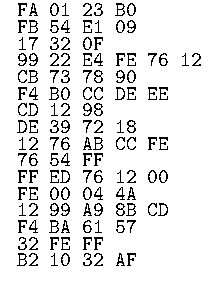
\includegraphics[scale=1.2]{cisc_code_hex}
\caption{Machine code in \code{HEX}.}
\label{figure:cisc_code_hex}
\end{figure}
\begin{choices}
\choice The size of the instruction memory.
\choice The number of clock cycles per instruction.
\choice The assembly code corresponds to a \acs{RISC}.
\choice All the above.
\CorrectChoice None of the above.
\end{choices}
\answer{0}{The code from~\fref{figure:cisc_code_hex} has variable-lenght encoding, which means that it corresponds to a \acs{CISC}.}

%\newpage
%% ========================================
%\question[20] Assume that a \acs{uP} supports the instructions
%\begin{center} 
%\code{ADD}, \code{D}, \code{S1}, \code{S2} \\
%\code{SUB}, \code{D}, \code{S1}, \code{S2}
%\end{center}
%for additions and subtractions, respectively.
%The destination \code{D} could be either a \code{Reg} or a \code{Mem} location. 
%Similarly, \code{S1} and \code{S2} correspond to the source of the operands and they may also be either a \code{Reg} or a \code{Mem} location.
%Assume the notation of addressing modes shown in~\tref{table:addressing_modes}.
%
%Using the registers and memory values shown in~\Cref{table:regs,table:mem}, respectively, complete \Cref{table:regs_fill,table:mem_fill} with the values of \code{Reg} and \code{Mem} after executing the operations shown in parts~\ref{part:address1} to~\ref{part:address4} of this question. 
%Assume operations are independent from each other, \ie, the order of execution is not important and the result of one operation does not affect the execution of the rest.
%
%\begin{table}[!h]
\centering
\caption{Memory addressing notation}
\label{table:addressing_modes}
\begin{tabular}{|c|c|}
\hline
Memory addressing & Notation \\
\hline\hline
Register          & \code{R}          \\\hline
Absolute          & \code{(constant)} \\\hline
Register indirect & \code{(R)}        \\\hline
Memory indirect   & \code{@(R)}       \\\hline
\end{tabular}
\end{table}
%\begin{minipage}[b]{0.45\hsize}
\centering
\captionsetup{type=table}
\captionof{table}{\code{Reg} values}
\label{table:regs}
  \begin{tabular}{c|c}
  \code{Reg} & \code{Value} \\\hline
  \code{R1}  & \code{3} \\ 
  \code{R2}  & \code{11} \\ 
  \code{R3}  & \code{19} \\ 
  \code{R4}  & \code{31} \\ 
  \end{tabular}
\end{minipage}
\hfill
\begin{minipage}[b]{0.45\hsize}
\centering
\captionsetup{type=table}
\captionof{table}{\code{Mem} values}
\label{table:mem}
  \begin{tabular}{c|c}
  \code{Mem} & \code{Value} \\\hline
  \code{11}  & \code{5} \\ 
  \code{17}  & \code{41} \\ 
  \code{19}  & \code{43} \\ 
  \code{23}  & \code{29} \\ 
  \code{31}  & \code{11} \\ 
  \code{37}  & \code{13} \\ 
  \code{41}  & \code{23} \\ 
  \code{43}  & \code{53} \\ 
  \code{53}  & \code{59} \\ 
  \end{tabular}
\end{minipage}
%
%\begin{parts}
%\part \code{SUB}, \code{R1},   \code{(23)}, \code{R2}\label{part:address1}
%\answer{0}{\code{R1} $\leftarrow$ \code{Mem[23] - R2} \\ 
%\code{R1} $\leftarrow$ \code{29 - 11} \\ 
%\code{R1} $\leftarrow$ \code{18} }
%\part \code{ADD}, \code{(17)}, \code{(R2)},  \code{@(R4)}\label{part:address2}
%\answer{0}{\code{Mem[17]} $\leftarrow$ \code{Mem[R2] + Mem[Mem[R4]]} \\
%\code{Mem[17]} $\leftarrow$ \code{Mem[11] + Mem[Mem[31]]} \\
%\code{Mem[17]} $\leftarrow$ \code{Mem[11] + Mem[11]} \\
%\code{Mem[17]} $\leftarrow$ \code{5 + 5} \\
%\code{Mem[17]} $\leftarrow$ \code{10}
%}
%\part \code{ADD}, \code{R2}, \code{(41)}, \code{R3}\label{part:address3}
%\answer{0}{\code{R2} $\leftarrow$ \code{Mem[41] + R3} \\
%\code{R2} $\leftarrow$ \code{23 + 19} \\
%\code{R2} $\leftarrow$ \code{42} \\}
%\part \code{SUB}, \code{@(R3)}, \code{(R4)}, \code{(11)}\label{part:address4}
%\answer{0}{\code{Mem[Mem[R3]]} $\leftarrow$ \code{Mem[R4] - Mem[11]} \\
%\code{Mem[Mem[19]]} $\leftarrow$ \code{Mem[31] - Mem[11]} \\
%\code{Mem[43]} $\leftarrow$ \code{Mem[31] - Mem[11]} \\
%\code{Mem[43]} $\leftarrow$ \code{11 - 5} \\
%\code{Mem[43]} $\leftarrow$ \code{6} }
%
%\renewcommand{\arraystretch}{2}
\begin{minipage}[b]{0.45\hsize}
\centering
\captionsetup{type=table}
\captionof{table}{\code{Reg} values}
\label{table:regs_fill}
  \begin{tabular}{c|c}
  \code{Reg} & Value \\
  \midrule
  \code{R1}  &  \\   \midrule
  \code{R2}  &  \\   \midrule
  \code{R3}  &  \\   \midrule
  \code{R4}  &  \\   \midrule
  \end{tabular}
\end{minipage}
\hfill
\begin{minipage}[b]{0.45\hsize}
\centering
\captionsetup{type=table}
\captionof{table}{\code{Mem} values}
\label{table:mem_fill}
  \begin{tabular}{c|c}
  \code{Mem} & Value \\
  \toprule
  \code{11}  &  \\   \midrule
  \code{17}  &  \\   \midrule
  \code{19}  &  \\   \midrule
  \code{23}  &  \\   \midrule
  \code{31}  &  \\   \midrule
  \code{37}  &  \\   \midrule
  \code{41}  &  \\   \midrule
  \code{43}  &  \\   \midrule
  \code{53}  &  \\   \midrule
  \end{tabular}
\end{minipage}
\renewcommand{\arraystretch}{1.0}
%
%\end{parts}

%\newpage
% ========================================
\question[4] Explain and give an example (using assembly code, for instance) of each of the following addressing modes.
\begin{enumerate}
\item Immediate.
\item Register.
\item Absolute.
\item Register indirect.
\end{enumerate}
\answer{\longanswerspace}{} 

% ========================================
\question[3] What is a benchmark?
\answer{\longanswerspace}{A set of computer programs designed for measured the performance, for example latency, of a \acs{uP} or a complete computing system.}  

% ========================================
\question[8] Assuming that the dynamic power of a microchip may be calculated with
\begin{equation}
P_{dyn} = \alpha \cdot C \cdot \VDD^{2} \cdot \fclk
\end{equation}
calculate the power saving of a \acs{uP} when its supply voltage is dropped to $85\%$ of its nominal supply and its clock period is increased by $20\%$. Since no calculators are allowed, please write down the expression you'd use in order to calculate the power saving.
\\\textbf{HINT.} Find the ratio $P_{2}/P_{1}$, where $P_{1}$ and $P_{2}$ are the nominal and improved dynamic powers, respectively.
\answer{\longanswerspace}{
$\VDDX{2}=0.85\cdot\VDDX{1}$\\
$\TclkX{2}=1.20\cdot\TclkX{1}$\\
$\fclkX{2}=\fclkX{1}/1.20$\\
$P_{2}/P_{1}=0.85^2/ 1.20$\\
$P_{2}/P_{1}=0.60208$
} 

% ========================================
\question[5] Name \textbf{AND} explain one of the three power saving techniques commonly used at the circuit level in \acsp{SoC}.
\answer{\longanswerspace}{Clock gating, power gating, dynamic voltage and frequency scaling.} 

% ========================================
\question[8] Using SystemVerilog (or Verilog) design a module that can provide the output Q of \fref{Figure:Clock_divider}.\label{Question:SV_clock_divider}
\begin{figure}[!h]
\centering
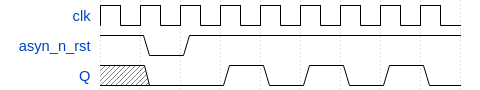
\includegraphics[width=\textwidth]{wavedrom/clk_div2}
\caption{Waveform for \qref{Question:SV_clock_divider}}
\label{Figure:Clock_divider}
\end{figure}
\answer{\longanswerspace}{} 

% ========================================
\newpage
\question[6] Design a SystemVerilog module for a D-type Flip-Flop with synchronous active-high reset.
\answer{\longanswerspace}{} 

% ========================================
\question[6] In SystemVerilog, what's the difference between blocking and non-blocking assignments and when/where do you use them?
\answer{\longanswerspace}{} 

% ========================================
\question[6] Explain what do we use ModelSim and Quartus for.
\answer{\longanswerspace}{} 

% ========================================
\question[5] The execution of a \acs{MIPS} \acs{uP} may be divided into different stages. Name \textbf{AND} explain each of all those stages. 
\answer{\longanswerspace}{
\begin{enumerate}
\item Instruction Fetch.
\item Instruction Decode.
\item Execute.
\item Memory Access.
\item Write Back.
\end{enumerate}
} 

% ========================================
\question[6] Explain each of the three types of instructions implemented in your \acs{MIPS} project.
\answer{\longanswerspace}{R-Type: Register-to-register\\
I-Type: Immediate-type instructions.\\
J-Type: Jump-type instructions.
}

% ========================================
\question[6] Explain what happens when an interrupt or exception occurs in a \acs{CPU}.
\answer{\longanswerspace}{
\begin{enumerate}
\item Value of PC is stored.
\item Control flow is granted to the handler by updating the PC with the interrupt/exception handler's address.
\item The handler executes its routine (program).
\item Flow control is returned to the main program by restoring the value of PC.
\end{enumerate}
}

% ========================================
\question[6] Explain the difference between an exception and an interrupt.
\answer{\longanswerspace}{Exceptions are synchronous unscheduled events that occur internally to the processor. By contrast, interrupts are synchronous events that occur externally to the processor.}

% ========================================
\question[2] An interrupt is a synchronous event that occur externally to the processor. 
\begin{choices}
\CorrectChoice False.
\choice True.
\end{choices}

% ========================================
\question[2] Select the correct answer.
\begin{choices}
\choice An arithmetic overflow may cause an interrupt.
\choice A timer may cause an exception.
\choice A key stroke is a predictable event. Hence it may be treated as an exception.
\choice An unsupported instruction may be treated as an interrupt.
\choice All of the above.
\CorrectChoice None of the above. 
\end{choices}

% ========================================
\question[2] This data structure may be used in order to store the return addresses of a program in a nested interrupts/exceptions scheme.
\begin{choices}
\choice First-In First-Out.
\choice RAM.
\CorrectChoice First-In Last-Out.
\choice Binary trees.
\end{choices}

% ========================================
\question[6] Thoroughly explain what pipeline is and how it is used in order to improve the performance of a \acs{uP}.
\answer{\longanswerspace}{}

% ========================================
\question[6] Explain each of the hazards associated with pipelining.
\answer{\longanswerspace}{Structural: A required resource is busy.\\ 
Data: Need to wait for previous instruction to complete its data read/write.\\
Control: Deciding on control action depends on previous instruction such as branches.
}

% ========================================
\question[6] Explain what a pipeline stall is and how it can be mitigated.
\answer{\longanswerspace}{A pipeline stall occurs when the pipeline needs to be stopped for one or more clock cycles. It effectively translates in the pipeline not performing any instruction. It can be mitigated with techniques such as forwarding (bypassing), code scheduling, branch prediction.
}
%\newpage
% ========================================
\question[10] Analyse the following assembly code for the \acs{MIPS} \acs{uP} you've designed. Write down the contents of \code{Mem[0]} to \code{Mem[5]} after the execution of the code. Assume that this is a single-cycle design, which means there are no pipeline hazards. Remember that \code{r0} is a constant 0. Also remember that \code{LWI} and \code{SWI} are absolute addressing modes, whilst \code{LWR} and \code{SWR} correspond to indirect register addressing modes.
\begin{table}[!ht]
\begin{tabular}{rllll}
~ & \code{LLI} & \code{r1,} & \code{5}\\
~ & \code{LLI} & \code{r2,} & \code{0}\\
~ & \code{LLI} & \code{r3,} & \code{1}\\
~ & \code{LLI} & \code{r4,} & \code{0}\\

~ & \code{SWR} & \code{r3,} & \code{(r1)}\\
~ & \code{ADD} & \code{r4,} & \code{r2,} & \code{r3}\\
\code{loop:} & \code{SUBI} & \code{r1,} & \code{1} \\
~ & \code{SWR} & \code{r4,} & \code{(r1)}\\
~ & \code{BEQ} & \code{r1,} & \code{r0,} & \code{end}\\
~ & \code{SWI} & \code{r3,} & \code{(100)}\\
~ & \code{LWI} & \code{r2,} & \code{(100)}\\
~ & \code{LWR} & \code{r3,} & \code{(r1)}\\
~ & \code{ADD} & \code{r4,} & \code{r2,} & \code{r3}\\
~ & \code{J} & \code{loop}\\
\code{end:} & J & \code{end}\\
\end{tabular}
\end{table}
\answer{\longanswerspace}{
}

% ========================================
\question[4] Select \textbf{ALL} the correct statements. Each correct answer will award you 2 pts. Each incorrect answer will deduct 1 pt. \begin{choices}
\choice Pipelining may decrease throughput.
\CorrectChoice Pipelining may increase latency.
\CorrectChoice Pipelining may increase throughput.
\choice Pipelining may decrease latency. 
\end{choices}

% ========================================
\question[2] Cache memories are usually implemented using \acsp{DRAM} since they are inexpensive.
\begin{choices}
\choice True.
\CorrectChoice False.
\end{choices}

% ========================================
\question[2] A single \acs{SRAM} cell requires less chip area than a single \acs{DRAM} cell.
\begin{choices}
\choice True.
\CorrectChoice False.
\end{choices}

% ========================================
\question[5] Explain what a cache memory is and what it is used for.
\answer{\longanswerspace}{}

% ========================================
\question[5] Explain what a cache miss is and what is the penalty associated with it.
\answer{\longanswerspace}{CPU needs to read/write data that is not in the cache and its penalty is that the data must be retrieved from an upper level of memory hierarchy, incurring in a delay and pipeline stall.
}

% ========================================
\question[5] Regarding cache memories, explain the basic idea of temporal and spatial locality.
\answer{\longanswerspace}{Temporal locality: Data accessed recently is likely to be accessed again soon.\\
Spatial locality: Data near data accessed recently is likely to be accessed soon.
}

% ========================================
\newpage
\question[2] In a direct mapped cache, any \acs{RAM} location may be allocated to any cache location. 
\begin{choices}
\CorrectChoice False.
\choice True.
\end{choices}

%% ========================================
\bonusquestion[5]\textbf{Bonus points question}. 
Who was the first man on space and what was his nationality? No partial credits will be granted.
\answer{\answerspace}{Yuri Alekseyevich Gagarin - Soviet/Russian.} 

%% ========================================
\bonusquestion[5]\textbf{Bonus points question}. 
What's the difference between Great Britain and United Kingdom? No partial credits will be granted.
\answer{\answerspace}{UK includes Northern Ireland} 

%% ========================================
%\question[5]\textbf{Bonus points question}. 
%On which date (day/month/year) did the first manned moon landing occur and what was the name of the mission? No partial credits will be granted.
%\answer{\answerspace}{Apollo 11, 20th July 1969.}  
%
%% ========================================
%\question[5]\textbf{Bonus points question 2}. 
%Name all the countries that comprise the United Kingdom and name the capital city of each of those countries. No partial credits will be granted.
%\answer{\answerspace}{England (London), Wales (Cardiff), Scotland(Edinburgh), Northern Ireland (Belfast).} 
                  
\end{questions}

\end{document}